\section{CNN Training}

\subsection{Data Preparation}

不仅是在CV当中,在诸如数据科学等学科之中,对数据进行分析之前通常要进行预处理 (processing).
以处理CIFAR-10的$32\times32\times3$数据集,我们有逐通道减去均值 (VGG)或逐通道减去均值然后除以标准差 (ResNet).

标准化有什么作用呢?例如,如果神经元的输入都是正数,那么权重的导数就会都是正的或者负的.而非标准化的数据可能具有很大的数值,
对于权重矩阵的微小变化非常敏感,难以训练.

\subsection{Weight Initialization}

\begin{figure}[htbp]
	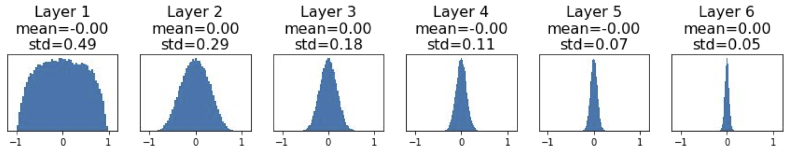
\includegraphics[scale=0.55]{figures/grad_var.png}
	\caption{梯度方差示意图}
	\label{grad_var}
\end{figure}

权重矩阵的初始化并不是一件随意的事情,它代表了我们优化的起点.一个最简单的想法是:用一些小的零均值随机数,
比如调用\texttt{0.01 * np.random.randn (Din, Dout)}生成参数矩阵.但是这样做,由于参数都是一些服从高斯分布的随机数,
这会导致梯度的方差逐层递减,最后梯度非常小,训练困难,如图所示\ref{grad_var}.

一个优化方法是每层都进行标准化,同时令参数的方差为 $\frac{1}{D_{in}}$.

数学推导:

假设 $y=x_1w_1+\cdots+x_nw_n$ ,我们希望 $Var(y)=Var(x_i)$,这样可以保证梯度的方差不会随着层数的增加而变小.那么:

\begin{equation}
	\begin{aligned}
		Var(y) &= Var(x_1w_1+\cdots+x_nw_n)
		\\
		&= Var(x_1w_1)+\cdots+Var (x_nw_n)
		\\
		&= Var(x_1)Var(w_1)+\cdots+Var(x_n)Var(w_n)
		\\
		&= n Var(x)Var(w)
		\\
		\Rightarrow Var(w)=\frac{1}{n}
	\end{aligned}
\end{equation}

在使用ReLu时,可以视为去掉一半神经元,参数方差为 $\sqrt{\frac{2}{D_{in}}}$.

\subsection{Start Optimization}

\begin{figure}[htbp]
	\centering
	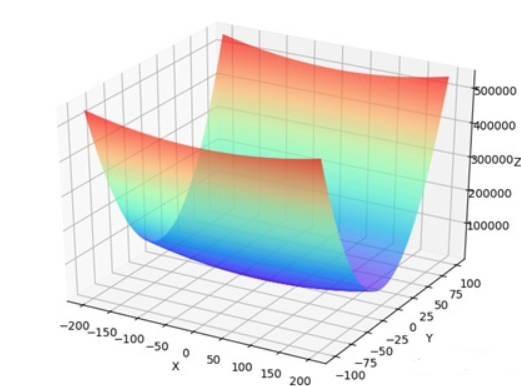
\includegraphics[scale=0.55]{figures/valley.png}
	\caption{山谷示意图}
	\label{valley}
\end{figure}

前面我们提到过用SGD的方法进行训练,但在矩阵的Condition Number\footnote{有关矩阵Condition Number的简单叙述,请见附录.}
较大的时候,SGD的效果仍然不够好.对SGD来说,山谷和鞍点仍然是巨大的麻烦.所谓山谷,
就是类似右图的地形\footnote{本小节的配图和叙述参考了@郑思座的\href{https://zhuanlan.zhihu.com/p/60088231}{这篇文章}.此文还介绍了牛顿动量法和自然梯度法.}:

如果梯度下降进入如图所示的地形,则由于山谷两侧的梯度指向谷底,因此如果山谷中比较平缓,
则很可能在两侧山壁来回打转,或需要很长时间才能到达谷底的最小值.

因此,在SGD的基础上我们可以添加动量方法 (Momentum)\footnote{为什么动量优化work?可以参考这个可视化可交互网站:\href{http://distill.pub/2017/momentum}{Why Momentum Really Works}},
所谓动量方法,就是对历史梯度进行记录,并以一定权重影响当前的梯度.

具体来说,结合物理学上的动量思想,在梯度下降问题中引入动量项$m$和折扣因子$\gamma$,公式变为 

\begin{equation}
	\begin{aligned}
		m &\leftarrow \gamma m+\eta \nabla_{\theta} \mathcal L(\theta)
		\\
		\theta &\leftarrow \theta-m
	\end{aligned}
\end{equation}

其中,$\gamma$表示历史梯度的影响力,$\gamma$越大,历史梯度对现在的影响也越大.
直观上来说,要是当前时刻的梯度与历史梯度方向趋近,这种趋势会在当前时刻加强,否则当前时刻的梯度方向减弱.

我们用SGD+Momentum来对图\ref{valley}进行梯度下降.下面分别是两个不同参数情形时的俯视图.
如果不加momentum,则可以想见点将会以近乎垂直于等高线的方向来回震荡.左图中每个较长的梯度下降之后,
跟着的一段较短并且一定程度矫正了方向,这正是历史梯度的作用.而右图则是$\gamma$较大的情形,
此时历史梯度的权重过大,积重难返,优化效果要差一些.

\begin{figure}[htbp]
	\centering
	\subfigure[$\eta=0.016, \gamma=0.7$]{
		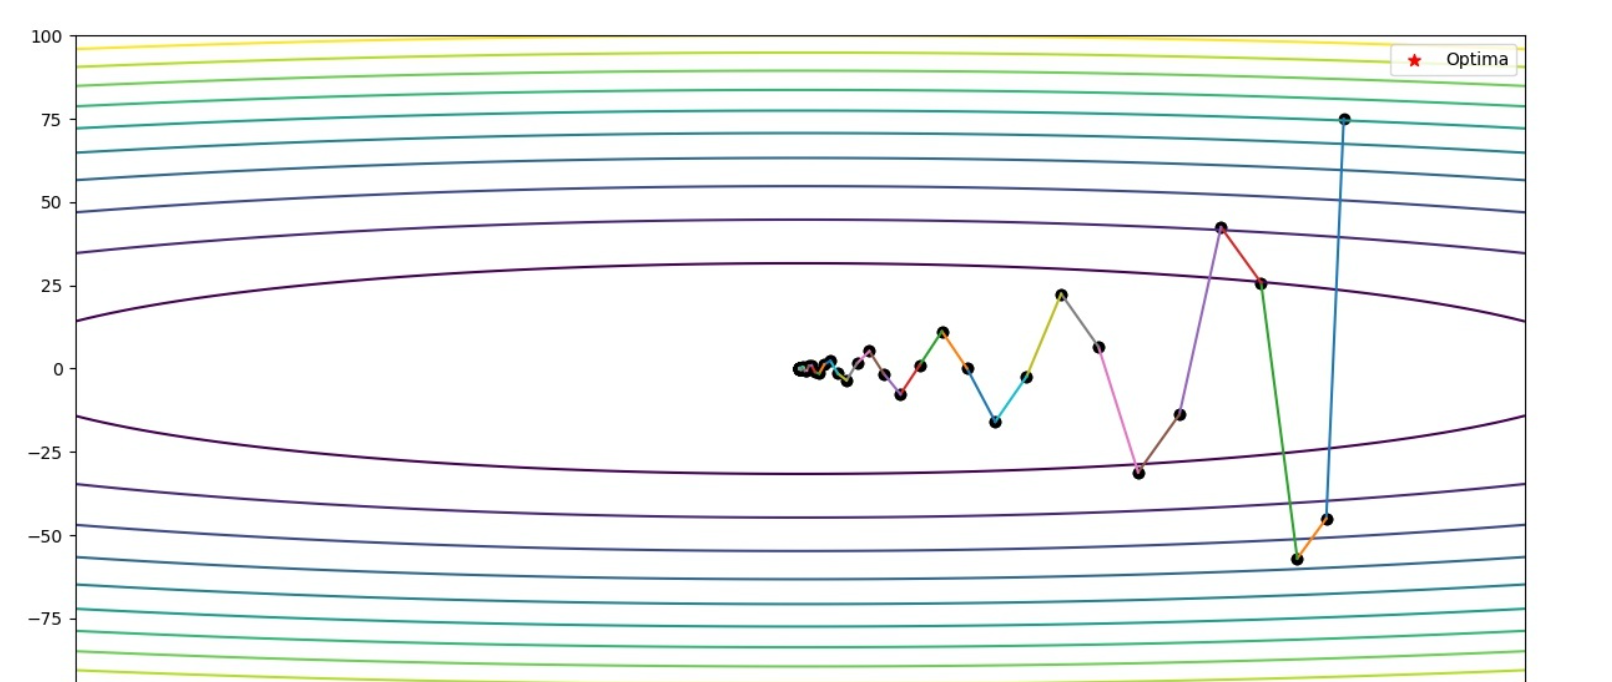
\includegraphics[scale=0.2]{figures/msgd1.png}
	}
	\subfigure[$\eta=0.016, \gamma=0.9$]{
		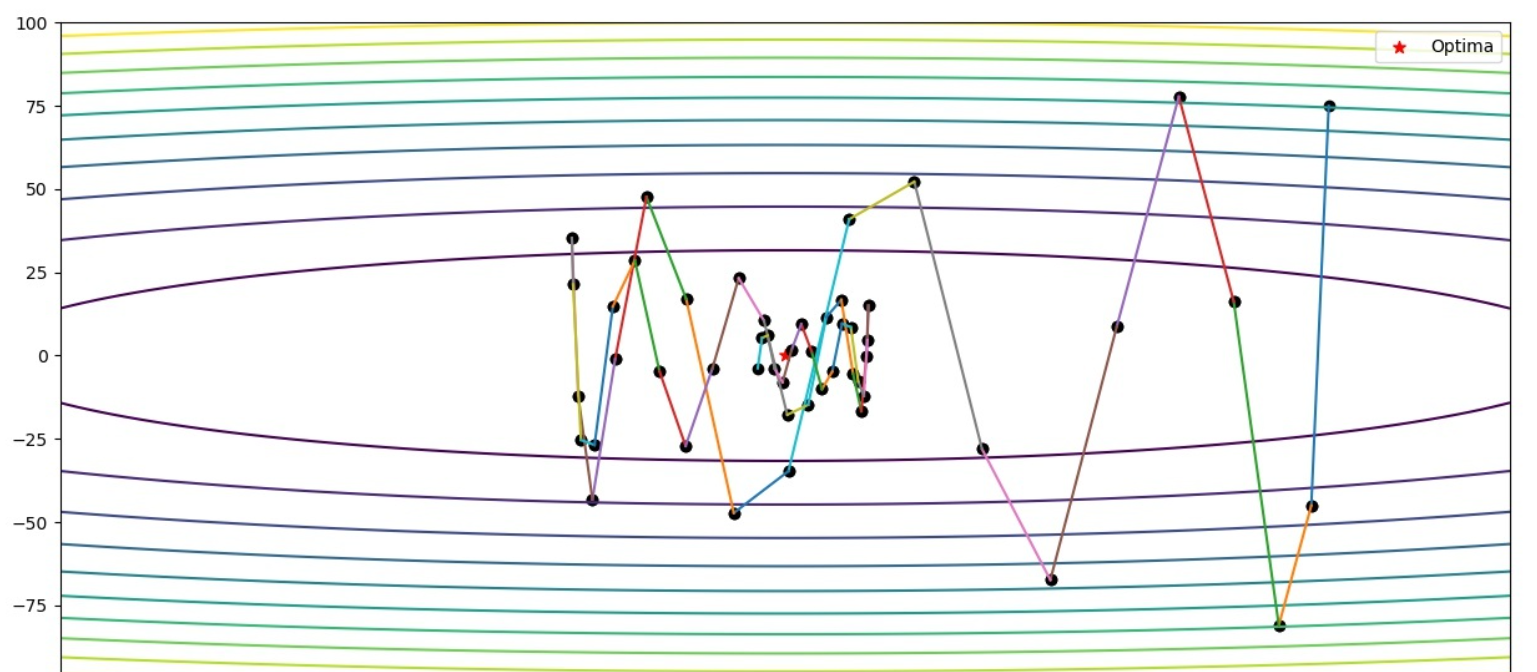
\includegraphics[scale=0.2]{figures/msgd2.png}
	}
\end{figure}

再来考察另一个麻烦:鞍点.存在鞍点意味着此处的 Hessian Matrix 有正负特征值,是不定的,
因而随机梯度下降很可能无法找到下降的方向.
由于深度学习实践中普遍维度较高,比如在1000维当中只有两个维度不是local minimum,
那么SGD也很难跳出这里.这也是偶尔会看到loss长时间不动而突然间骤减的可能原因.

若用$G_{t}$表示第$t$轮迭代的动量,$g_{t}=\eta \nabla_{\theta} \mathcal L(\theta)$
表示第$t$轮迭代的更新量,当$t \rightarrow \infty , G_{\infty}=\frac{g_{0}}{1-\gamma}$,
该式的含义是如果梯度保持不变,最终的更新速度会是梯 度项乘以学习率的$\frac{1}{1-\gamma}$倍.
举例来说,$\gamma=0.9$时,动量算法最终的更新速度是普通梯度下降法 的10倍,意味着在穿越"平原" 
和"平缓山谷"从而摆脱局部最小值时,动量法更有优势.

在书写代码时,我们通常这样写:

\begin{equation}
	\begin{aligned}
		v_{t+1} &\leftarrow \rho v_{t} + \nabla f(x_t)
		\\
		x_{t+1} &\leftarrow x_t - \alpha v_{t+1}
	\end{aligned}
\end{equation}

也就是将velocity项作为梯度的运行时均值.一般取$\rho = 0.9$或$\rho = 0.99$.

Adam就是一种应用了Momentum的优化方法.具体如下图.

\begin{figure}[htbp]
	\centering
	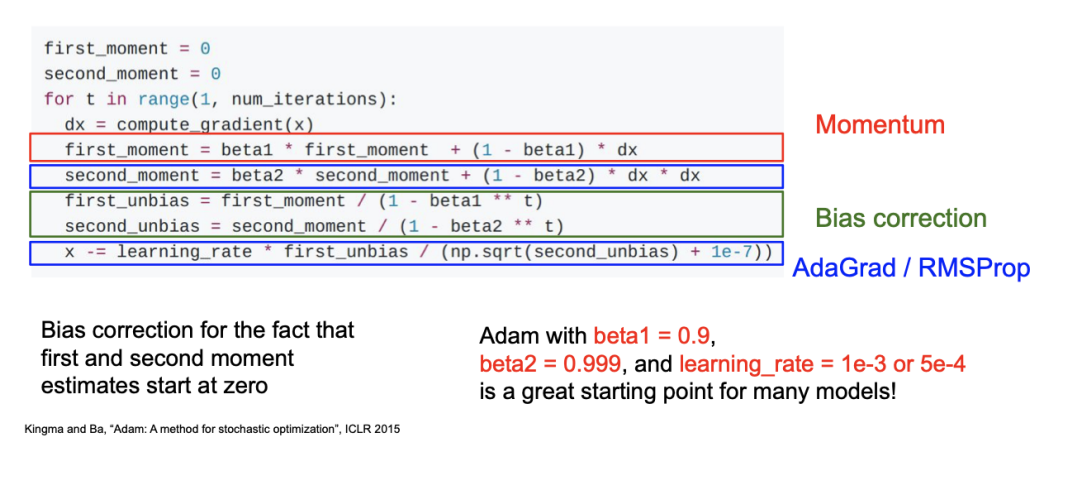
\includegraphics[scale=0.65]{figures/adam.png}
	\caption{Adam}
\end{figure}

\subsection{Learning Rate Schedule}

在神经网络的训练过程中,如何设定学习率的变化策略也是很重要的,因为越靠近最小值,其对学习率的取值可能越敏感,
需要更加精细地取值.我们先来看一张不同大小的学习率对于loss function的影响.
\sout{由此可以看出,好的学习率就应该像临界阻尼一样,让阻尼振荡又快又稳地回到平衡位置...(胡言乱语)}

\begin{figure}[htbp]
	\centering
	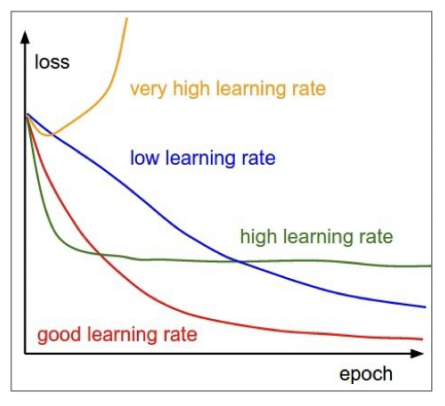
\includegraphics[scale=0.65]{figures/learning_rate_schedule.png}
	\caption{不同学习率对损失函数的影响}
\end{figure}

较低的学习率会使得训练所需时间较长,而过高的学习率会限制最终的结果.如果学习率非常高,可
能loss反而会上升\footnote{这里老师在课上说不一定,并提问:对于 classification 问题,也会上升吗?
有想法的同学欢迎联系笔者,我将在此添加您的真知灼见.
两年之后的笔者对这个问题也没有想法orz}.

一种策略是,在固定轮数之后,缩减学习率.比如ResNet在每30个epoch
\footnote{此处王鹤老师详细解释了iteration和epoch两个概念的区别.一次iteration,
就是跑完一次mini-batch的过程.而epoch的含义则更加灵活.它可指代:1.训练完整个dataset称为一个epoch.
例如将3200张图片分为100个mini-batch,则1 epoch = 100 iteration.  2.每个epoch结束保存一次模型.  
3.epoch作为绘制curve的单元.  4.进行model evalidation的单元.}后将学习率乘以$0.1$.
除此之外还有多种形式,如余弦,线性递减,除以轮数的平方根等.

除了一定轮数之后的递减策略,在训练伊始,也有"热身"的递增策略.过高的初始学习率对优化会产生不利影响,
但在约前5000次迭代中线性增长学习率可以避免这种影响.另外,有一个经验定律:如果将batch的大小增长了$N$,
那么学习率也变为$N$倍.

总之,对于学习率策略而言,Adam+默认学习率在多数情形下都是一个默认较好的选择,甚至它对于常数学习率也常常运行得不错.
而SGD+Momentum的组合可以取得比Adam更好的效果,但恐怕要在学习率策略上花费更多头发.
(余弦函数是个不错的较少参数的策略.)